% ----------------------------------------------------------
\chapter{Resultados de Simulação}\label{cap:resultados}
% ----------------------------------------------------------

O objetivo desse capítulo é a implementação da estratégia de controle desenvolvida no Capítulo \ref{cap:descricao-controle} utilizando a modelagem matemática descrita no Capítulo \ref{cap:modelo} para a seção típica apresentada por \textcite{book:Fung}. Os parâmetros do sistema são mostrados na Tabela \ref{tab:parametros-secao-tipica}.

\begin{table}[h]
\centering
\caption{Parâmetros do sistema}
\begin{tabular}{ccc}
Parâmetro   & Valor & Unidade                 \\ \hline
$m$ & 0,120 & kg \\
$b$ & 0,127 & m  \\
$a$ & -0,15 & - \\
$e$ & 0,30  & - \\
$I_{\theta}$ & $7,500\cdot10^{-4}$ & $\text{kg} \cdot \text{m}^{2}$ \\
$S_{\theta}$ & $3,804\cdot10^{-3}$ & $\text{kg} \cdot \text{m}$  \\
$S_{\delta,h}$ & $3,804\cdot10^{-3}$ & $\text{kg} \cdot \text{m}$  \\
$S_{\delta,\theta}$ & $5.891\cdot10^{-5}$ & $\text{kg} \cdot \text{m}^{2}$ \\
$\omega_{h}$ & 55,92 & rad/s \\
$\omega_{\theta}$ & 64,10 & rad/s \\
$\xi_{h}$ & 0,05 & - \\
$\xi_{\theta}$ & 0,05 & - \\ \hline
\end{tabular}
\label{tab:parametros-secao-tipica}
\end{table}

A velocidade de \textit{flutter} em malha aberta será denominada \gls{VOLF} no restante desse capítulo, e o valor de referência, calculado por \textcite{book:Fung}, é igual à $29,9$ m/s. 

As análises apresentadas nas seções subsequentes foram realizadas para a condição de voo \glsxtrfull{ISA}, ao nível do mar.

% ----------------------------------------------------------

% ----------------------------------------------------------
\section{Matrizes Aerodinâmicas e Aproximação por funções racionais}\label{sec:resultados-aerodinamicos}

Consideraram-se $20$ valores de frequências reduzidas para a representação da aerodinâmica não-estacionária e construção das matrizes $\boldsymbol{AIC}$, modelada utilizando-se a função de \textit{Theodorsen}, como proposta por \textcite{book:Bisplinghoff}. Essa metodologia encontra-se detalhada no Apêndice A. Os valores de frequência reduzidas utilizados são mostrados na Tabela \ref{tab:reducedFrequencies}.

\begin{table}[h]
\centering
\caption{Frequências reduzidas para cálculo dos esforços aerodinâmicos}
\begin{tabular}{cccc} \hline
$k_{1} = 0,05$ & $k_{6} = 0,30$ & $k_{11} = 0,60$ & $k_{16} = 1,20$ \\
$k_{2} = 0,10$ & $k_{7} = 0,35$ & $k_{12} = 0,70$ & $k_{17} = 1,40$ \\
$k_{3} = 0,15$ & $k_{8} = 0,40$ & $k_{13} = 0,80$ & $k_{18} = 1,60$ \\
$k_{4} = 0,20$ & $k_{9} = 0,45$ & $k_{14} = 0,90$ & $k_{19} = 1,80$ \\
$k_{5} = 0,25$ & $k_{10} = 0,50$ & $k_{15} = 1,00$ & $k_{20} = 2,00$ \\ \hline
\end{tabular}
\label{tab:reducedFrequencies}
\end{table}

\newpage
Com a matrizes aerodinâmicas \gls{AICa} e \gls{AICc} determinadas, utilizou-se a metodologia apresentada na Seção \ref{sec:rfa-solucao} para aproximação dos esforços aerodinâmicos e representação no tempo. Foram adotados quatro termos de atraso, cujos valores encontrados que melhor ajustam a soma de funções racionais para o conjunto de frequências reduzidas utilizadas são mostrados na Tabela \ref{tab:lagParameters}. Esses parâmetros foram variados para encontrar o conjunto que melhor aproxima as matrizes \gls{RFA}s das matrizes \gls{AICa} e \gls{AICc} para todos os pontos de frequência reduzida nas quais essas matrizes foram determinadas.

\begin{table}[ht]
\centering
\caption{Termos de atraso aerodinâmico para aproximação $\textit{RFA}$}
\begin{tabular}{cccc}
Termo de atraso & Valor adotado \\ \hline
$p_{1}$ & 0,20 \\
$p_{2}$ & 0,40 \\
$p_{3}$ & 0,60 \\
$p_{4}$ & 0,80 \\ \hline
\end{tabular}
\label{tab:lagParameters}
\end{table}

Na Figura \ref{fig:RFAsModes} é mostrada uma comparação do termos das matriz $\boldsymbol{AIC}_{A}$ obtida e a \gls{RFA}, e percebe-se que há a uma similaridade para todos os pontos de frequência reduzida adotadas, garantindo uma aproximação satisfatória da aerodinâmica não estacionária para o modelo.

\begin{figure}[!h]
    \centering
    \caption{Comparação dos termos aerodinâmicos \gls{AICa} com a aproximação por \gls{RFA}}
    \noindent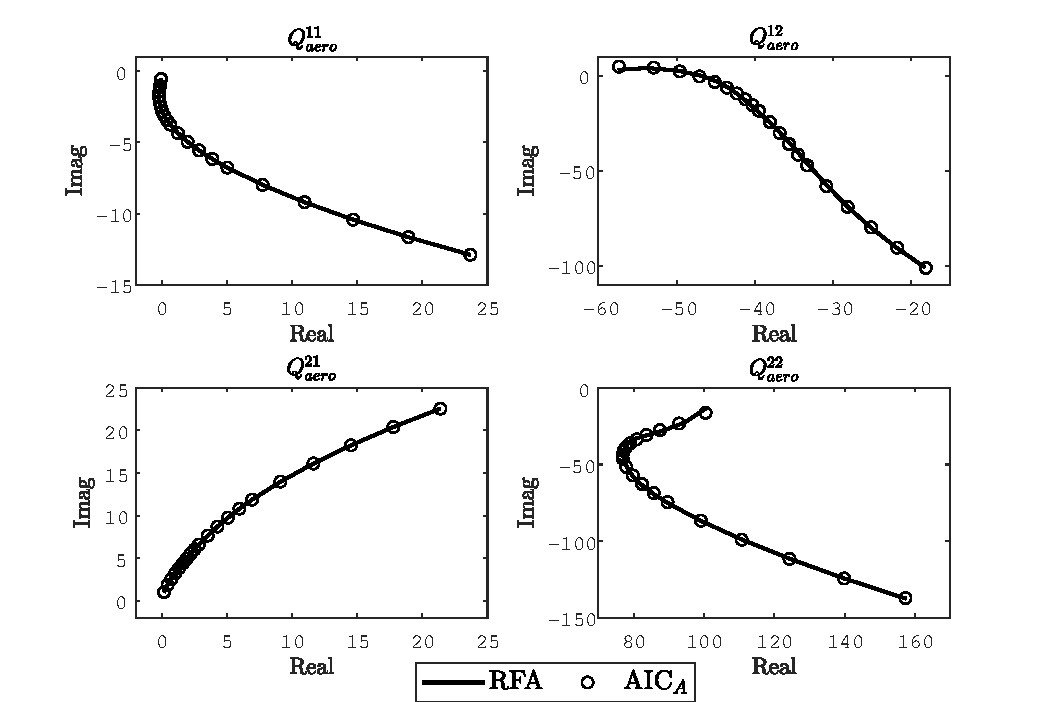
\includegraphics[width=\textwidth]{trabalho-graduacao/capitulos/figures/cap_4/RFAs/RFA_Modes.pdf}
    \label{fig:RFAsModes}
\end{figure}

\newpage

A aproximação dos termos aerodinâmicos referentes à superfície de controle, matriz $\boldsymbol{AIC}_{c}$, é apresentada na Figura \ref{fig:RFAsControl}. Destaca-se que os termos de aproximação também representam de forma apropriada o comportamento aerodinâmico não-estacionário para o movimento da superfície de controle.

\begin{figure}[ht!]
    \centering
    \caption{Comparação dos termos aerodinâmicos \gls{AICa} com a aproximação por \gls{RFA}}
    \noindent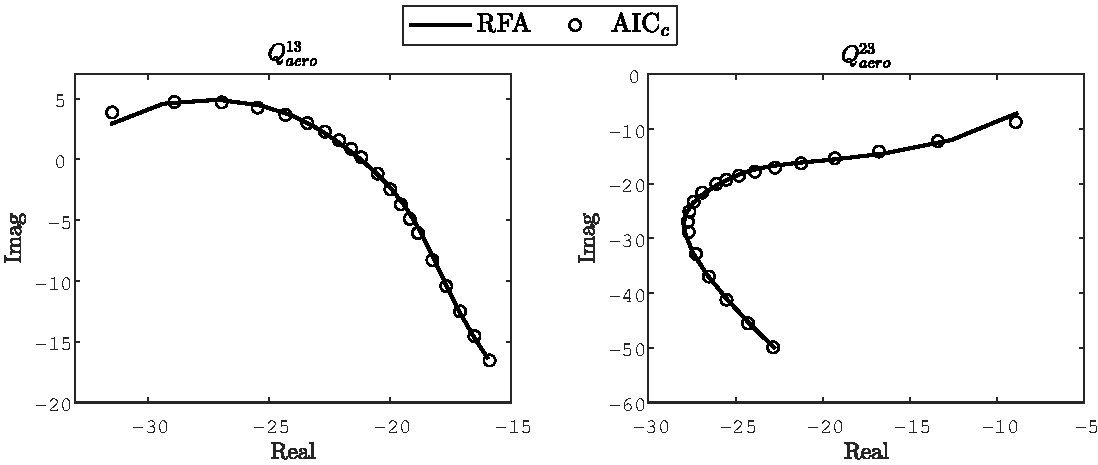
\includegraphics[width=\textwidth]{trabalho-graduacao/capitulos/figures/cap_4/RFAs/RFA_Control.pdf}
    \label{fig:RFAsControl}
\end{figure}
% ----------------------------------------------------------




% ----------------------------------------------------------
\section{Estabilidade em Malha Aberta}\label{sec:malha-aberta}

Após a determinação das matrizes de aproximação aerodinâmica, o modelo matemático no espaço de estados pode ser construído e a dinâmica do sistema avaliada. 

Inicialmente, um estudo da estabilidade em malha aberta do sistema foi realizado a partir do lugar geométrico das raízes para variação da velocidade do escoamento incidindo sobre a seção típica. Dessa forma, a velocidade de \textit{flutter} pode ser estimada como o valor na qual o lugar geométrico das raízes do sistema passe da região estável para a instável, isto é, do semiplano esquerdo para o direito do plano complexo.

Os resultado obtidos são apresentados na Figura \ref{fig:OpenLoop-Poles}, na qual pode ser observada a movimentação do conjunto de polos do sistema para diferentes velocidades. Destacada na figura está a velocidade de \textit{flutter}, como o ponto onde a parte real do respectivo polo é nula, representando a instabilidade do sistema para velocidades superiores à essa. Obteve-se o ponto de instabilidade do sistema como $V_{OLF} = 29,59$ m/s, corroborando o valor de velocidade de \textit{flutter} indicado por \textcite{book:Fung} para o respectivo modelo, com um erro inferior a $2\%$.

\begin{figure}[ht]
    \centering
    \caption{Lugar geométrico das raízes do sistema em malha aberta}
    \noindent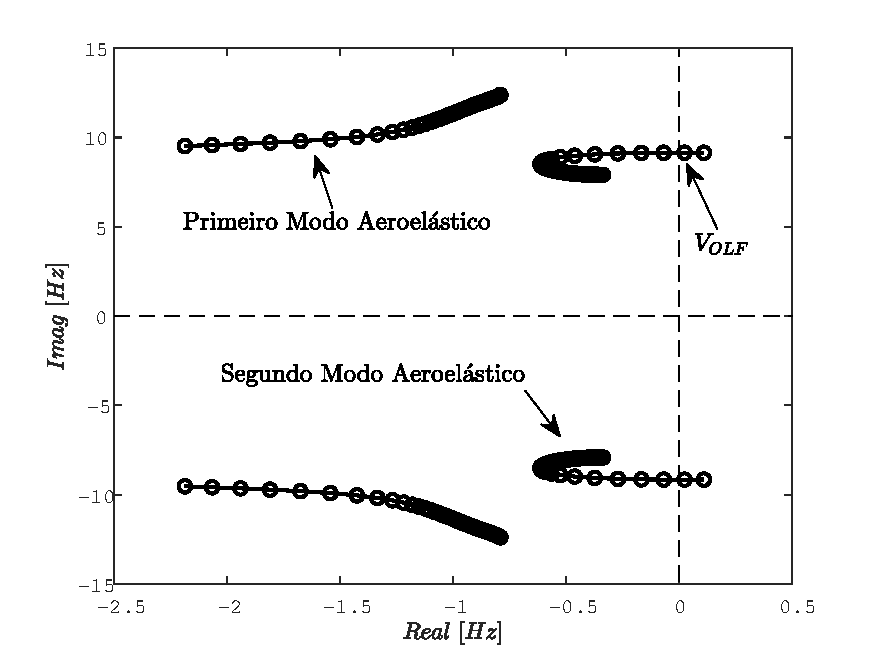
\includegraphics[width=\textwidth]{trabalho-graduacao/capitulos/figures/cap_4/Open-Loop/OpenLoop-Poles.pdf}
    \label{fig:OpenLoop-Poles}
\end{figure}

\newpage

Os polos referentes aos estados de atraso aerodinâmico foram omitidos devido ao desejo de destacar os polos que representam modos físicos do modelo, porém são apresentados na Tabela \ref{tab:VOLF-Poles}. As matrizes dinâmica, de entrada do sistema para a condição de \textit{flutter} em malha aberta, $V_{OLF} = 29,59$ m/s, foram obtidas como

\[
\boldsymbol{A} = 
\begin{bmatrix}
	\boldsymbol{0}_{2 \times 2} & \boldsymbol{I}_{2 \times 2}   & \boldsymbol{0}_{2 \times 8}   & \boldsymbol{0}_{2 \times 3} 	\\
	\boldsymbol{A}_{1} 	        & \boldsymbol{A}_{2} 	        & \boldsymbol{A}_{3} 	        & \boldsymbol{A}_{4} 		    \\
	\boldsymbol{0}_{8 \times 2} & \boldsymbol{A}_{5}  	        & \boldsymbol{A}_{6}	        & \boldsymbol{A}_{7}		    \\
	\boldsymbol{0}_{3 \times 2} & \boldsymbol{0}_{3 \times 2}   & \boldsymbol{0}_{2 \times 8}   & \boldsymbol{A}_{8}		    \\
\end{bmatrix}, \ \boldsymbol{B} = \begin{bmatrix}  \boldsymbol{0}_{14 \times 1} \\ 6,697\cdot10^{6} \end{bmatrix}
\]

\noindent onde as matrizes $\boldsymbol{A}_{i}$, sendo $i=1, 2, \cdots, 8$, que definem a matriz dinâmica $\boldsymbol{A}$ são dadas por

\[
\boldsymbol{A}_{1} = 
\begin{bmatrix}
-3682,960 & -3635,719 \\
476,618 & -2410,689
\end{bmatrix}, \ 
\boldsymbol{A}_{2} = 
\begin{bmatrix}
-11,014 & -14,789 \\
1,976 & -7,860
\end{bmatrix}
\]

\[
\boldsymbol{A}_{3} = 
\begin{bmatrix}
    133,688 & -17,283 & 133,688 & -17,283 & 133,688 & -17,283 & 133,688 & -17,283 \\
    -17,277 & 13,895 & -17,277 & 13,895 & -17,277 & 13,895 & -17,277 & 13,895
\end{bmatrix}
\]

\[
\boldsymbol{A}_{4} = 
\begin{bmatrix}
    -4,676 & -191,056 & 0,062 \\
    0,512 & -48,397 & 0,071
\end{bmatrix}, \
\boldsymbol{A}_{5} = 
\begin{bmatrix} 
    0,834 & 36,040      \\
    1,459 & -63,069     \\
    0,382 & -62,820     \\
    0,668 & 109,935     \\
    -1,085 & 94,801     \\
    1,898 & -165,902    \\
    0,073 & -47,649     \\
    0,128 & 83,387      \\
\end{bmatrix}
\]

\[
diag\left( \begin{bmatrix} -46,6 & -46,6 & -93,2 & -93,2 & -139,8 & -139,8 & -186,4 & -186,4 \end{bmatrix} \right)
\]

\[
\boldsymbol{A}_{7} = 
\begin{bmatrix}
    0 & 20,685  &  0 \\
    0 & -36,198 &  0 \\
    0 & -34,938 &  0 \\
    0 & 61,141  &  0 \\
    0 & 53,255  &  0 \\
    0 & -93,196 &  0 \\
    0 & -26,274 &  0 \\
    0 & 45,980  &  0 \\
\end{bmatrix}, \ 
\boldsymbol{A}_{8} = 
\begin{bmatrix}
    0 & 1 & 0 \\
    0 & 0 & 1 \\
    -6,697\cdot10^{6} & -5,330\cdot10^{4} & -2,827\cdot10^{2}
\end{bmatrix}
\]

\begin{table}[h]
\centering
\caption{Polos do sistema em malha aberta para velocidade $V_{OLF} = 29,59$ m/s}
\begin{tabular}{ccc} 
Polo em malha fechada & Valor do polo & Relação com variável de estado \\ \hline
$p_{1} $  & $0+0,575i$ & primeiro \gls{GDL}, $h$                                \\
$p_{2} $  & $0-0,575i$ & primeiro \gls{GDL}, $h$                                \\
$p_{3} $  & $-0,128+0,603i$ & segundo \gls{GDL}, $\theta$                       \\
$p_{4} $  & $-0,128-0,603i$ & segundo \gls{GDL}, $\theta$                       \\
$p_{5} $  & $-1,941+0i$ &  atraso aerodinâmico devido à \gls{RFA}          \\
$p_{6} $  & $-1,142+0,176i$ & atraso aerodinâmico devido à \gls{RFA}       \\
$p_{7} $  & $-1,142-0,176i$ & atraso aerodinâmico devido à \gls{RFA}       \\
$p_{8} $  & $-0,370+0i$ & atraso aerodinâmico devido à \gls{RFA}           \\
$p_{9} $  & $-1,864+0i$ & atraso aerodinâmico devido à \gls{RFA}           \\
$p_{10} $ & $-1,398+0i$ & atraso aerodinâmico devido à \gls{RFA}           \\
$p_{11} $ & $-0,932+0i$ & atraso aerodinâmico devido à \gls{RFA}           \\
$p_{12} $ & $-0,466+0i$ & atraso aerodinâmico devido à \gls{RFA}           \\
$p_{13} $ & $-1,885+0i$ & movimento da superfície de controle                   \\
$p_{14} $ & $-0,471+1,825i$ & movimento da superfície de controle               \\
$p_{15} $ & $-0,4712-1,825i$ & movimento da superfície de controle              \\
\hline
\end{tabular}
\label{tab:VOLF-Poles}
\end{table}

\newpage

Na Figura \ref{fig:OpenLoopSimulation}, é apresentada a resposta dinâmica do sistema no domínio do tempo, obtidos a partir de simulações numéricas em malha aberta, para uma condição inicial de $0,127$ m no primeiro grau de liberdade. A condição inicial imposta emula uma perturbação vista pelo sistema em relação à sua condição de equilíbrio e seu valor foi definido igual o parâmetro de meia corda do sistema.

Como esperado, para a condição de velocidade igual à velocidade de \textit{flutter} resultante da análise de estabilidade, a resposta dinâmica do sistema não mostra amortecimento da vibração estrutural. O resultado de simulação numérica alinhado com a análise de estabilidade em malha aberta a capacidade do modelo numérico desenvolvido de capturar a dinâmica do sistema não somente para movimentos oscilatórios desenvolvidos, mas garantindo representatividade na região transiente, como nos primeiros instantes de simulação apresentados na figura acima.

\begin{figure}[ht]
    \centering
    \caption{Simulação em malha aberta, para uma velocidade $V_{\infty} = 29,59$ m/s}
    \noindent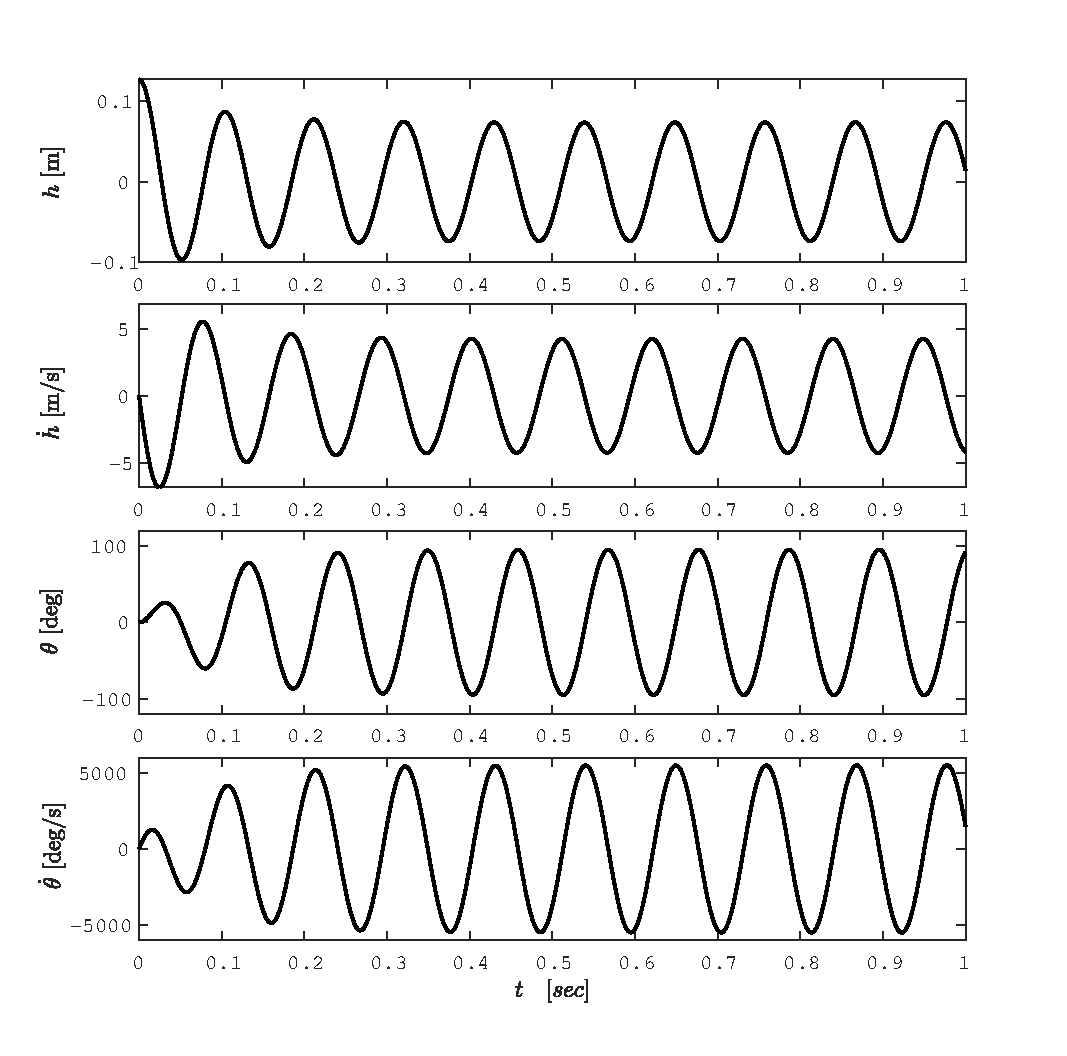
\includegraphics[width=0.95\textwidth]{trabalho-graduacao/capitulos/figures/cap_4/Open-Loop/OpenLoop-Simulation.pdf}
    \label{fig:OpenLoopSimulation}
\end{figure}


% ----------------------------------------------------------

% ----------------------------------------------------------
\section{Resultados em malha fechada}\label{sec:malha-fechada}

O modelo matemático calculado para a condição de $V_{OLF}$ foi utilizado para o desenvolvimento da lei de controle por realimentação de estados.

Para isso, inicialmente realizou-se a discretização do modelo para contabilizar os efeitos de amostragem no projeto da lei de controle. Adotou-se um período de amostragem igual à $0,01$ s, obtendo-se as matrizes do sistema digital como

\[
    \boldsymbol{\Phi} = \begin{bmatrix}
        \boldsymbol{\phi}_{1} & \boldsymbol{\phi}_{2} & \boldsymbol{\phi}_{3} \\
        \boldsymbol{\phi}_{4} & \boldsymbol{\phi}_{5} & \boldsymbol{\phi}_{6} \\
        \boldsymbol{\phi}_{7} & \boldsymbol{\phi}_{8} & \boldsymbol{\phi}_{9}
    \end{bmatrix}, \quad
    \boldsymbol{\Gamma} = \begin{bmatrix}  
    -0,288 \\ -0,105 \\ -88,008 \\ -30,247 \\ 5,542 \\ -9,699 \\ 
    -7,728 \\ 13,523 \\ 10,486 \\ -18,351 \\ -4,418 \\ 7,731  \\ 
    0,483 \\ 97,622 \\ 3,768\cdot10^{3}  
    \end{bmatrix}
\]

\noindent sendo as matrizes $\boldsymbol{\phi}_{i}$, para $i=1,2,\cdots,9$, definidas para melhor visualização como

\[
\boldsymbol{\phi}_{1} = 
\begin{bmatrix}
    0,827   & 0,164     & 0,009     & 0,001     & 0,005 \\
    0,021   & 0,884     & 0         & 0,009     & 0,001 \\
   -32,985  & -30,453   & 0,719     & 0,146     & 0,946 \\
    3,721   & -22,557   & 0,039     & 0,775     & 0,105 \\
    0,762   & -3,481    & 0,001     & 0,260     & 0,604 \\
\end{bmatrix}
\]

\[
\boldsymbol{\phi}_{2} = 
\begin{bmatrix}
    0,001 & 0,005 & 0,001 & 0,004 & 0,001 \\
    0,001 & 0,001 & 0     & 0     & 0     \\
    0,130 & 0,761 & 0,105 & 0,623 & 0,086 \\
    0,098 & 0,083 & 0,078 & 0,067 & 0,064 \\
    0,018 & 0,020 & 0,015 & 0,018 & 0,013 \\
\end{bmatrix}, \ 
\boldsymbol{\phi}_{3} = 
\begin{bmatrix}
    0,004 & 0      &  0,288 & 0,006 & 0      \\
    0     & 0      &  0,105 & 0,001 & 0      \\
    0,518 & 0,072  & 87,966 & 0,582 & 0,002  \\
    0,055 &  0,053 & 30,251 & 0,148 & 0,001  \\
    0,015 &  0,012 & -5,541 &  0,031 &  0    \\
\end{bmatrix}
\]


\[
\boldsymbol{\phi}_{4} = 
\begin{bmatrix}
   -1,334 &  6,092 &  0,001 & 0,455 &  0,041 \\
   -1,012 &  5,406 & 0,006 & 0,365 &  0,031 \\
    1,772 & -9,461 &  0,010 &  0,639 & 0,054 \\
    1,394 & -7,114 &  0,006 &  0,452 & 0,042 \\
   -2,440 & 12,450 & 0,010 & 0,791 &  0,074
\end{bmatrix}
\]

\[
\boldsymbol{\phi}_{5} = 
\begin{bmatrix}
 0,597 &  0,035 & 0,027 &  0,031 & 0,023 \\
 0,026 &  0,420 & 0,022 &  0,023 & 0,019 \\
 0,046 & 0,046 &  0,433 & 0,040 &  0,034 \\
 0,035 & 0,036 &  0,029 &  0,216 &  0,025 \\
 0,060 &  0,063 & 0,052 &  0,054 &  0,202
\end{bmatrix}, \ 
\boldsymbol{\phi}_{6} = 
\begin{bmatrix}
 0,027 & 0,021 &  9,698 & 0,055 & 0       \\
 0,020 & 0,017 &  7,726 & 0,023 & 0       \\
 0,035 &  0,030 & -13,521 & 0,041 &  0    \\
 0,027 &  0,022 & -10,485 & 0,015 &  0    \\
 0,047 & 0,039 & 18,349 & 0,026 & 0
\end{bmatrix}
\]


\[
\boldsymbol{\phi}_{7} = 
\begin{bmatrix}
    0,572 &  3,217 & 0,005 & 0,189 & 0,017 \\
    1,001 & -5,630 & 0,008 & 0,331 & 0,030 \\
    0 &  0 &  0 &  0 &  0 \\
    0 &  0 &  0 &  0 &  0 \\
    0 &  0 &  0 &  0 &  0
\end{bmatrix}\]

\[ 
\boldsymbol{\phi}_{8} = 
\begin{bmatrix}
 0,015 &  0,015 & 0,013 & 0,013 & 0,011 \\
 0,026 & 0,026 &  0,022 & 0,022 & 0,019 \\
 0 &  0 &  0 &  0 &  0 \\
 0 &  0 &  0 &  0 &  0 \\
 0 &  0 &  0 &  0 &  0 
\end{bmatrix}
\]

\[
\boldsymbol{\phi}_{9} = 
\begin{bmatrix}
 0,166 & 0,010 &  4,417 &  0,002 & 0         \\
 0,019 &  0,172 & -7,730 & 0,004 &  0      \\
 0 &  0 &  0,517 &  0,005 &  0             \\
 0 &  0 & -97,622 & 0,260 &  0,001         \\
 0 &  0 & -3768,616 & -127,611 & 0,419
\end{bmatrix}
\]


Para projetar a lei de controle, definiram-se os pesos como

\[    
\boldsymbol{W}_{x} = 1\cdot10^{3}\boldsymbol{I}_{N_{x}};  \quad \boldsymbol{W}_{u} = 1
\]

O problema do \gls{LQR} foi resolvido utilizando o \textit{software} MatLab, encontrando-se

\[
\begin{split}
\boldsymbol{K} &= 
[\begin{matrix} 1,942 &  8,956 & -0,070 & -0,027 & -0,116 & -0,005 & -0,088 &  0,001 & -0,064 \end{matrix} \\
&\qquad\qquad\qquad\qquad \begin{matrix} 0,002 & -0,049 &  0,002 & -999,877 & -9,283 & -0,019 \end{matrix}]
\end{split}
\]

Além de resultados de simulação, avaliou-se a evolução dos polos de malha fechada para variações na velocidade de \textit{flutter} utilizando o lugar geométrico das raízes (vide Figura \ref{fig:ClosedLoop-Poles}). Como pode ser observado, o controlador garante a estabilização do sistema na condição de $V_{OLF}$, condição de projeto da lei de controle. Mais ainda, a estabilidade é mantida até $\gls{VCLF}=31,37$ m/s. Apesar do aumento em $6 \%$ da velocidade de \textit{flutter} do sistema em malha fechada quando comparado à original, a introdução da estrutura de controle para supressão de \textit{flutter} não apresenta garantia de estabilidade para velocidades acima da de projeto, sendo esse aumento percentual uma consequência sem garantia teórica.

Para estabilizar o sistema na nova velocidade de flutter $\gls{VCLF}$, um novo modelo no espaço de estados deve ser calculado, o que torna necessário recalcular as matrizes de aproximação aerodinâmica. De posse do novo modelo, projeta-se um novo controlador por realimentação de estados. Então, durante a operação,  chaveia-se para o novo vetor de realimentação de estados quando o sistema estiver suficientemente próximo de tal velocidade. Alternativamente uma abordagem de escalonamento de ganhos poderia ser adotada para suavizar a transição entre diferentes pontos de operação.

Os valor dos polos em malha fechada para a velocidade $\gls{VCLF}$ são apresentados na Tabela \ref{tab:VOLF-ClosedLoop-Poles}.

\begin{table}[h]
\centering
\caption{Polos do sistema discreto em malha fechada para velocidade de \textit{flutter} em malha aberta ($V_{OLF} = 29,59$ m/s)}
\begin{tabular}{ccc} 
Polo em malha fechada & Valor do polo & Relação com variável de estado \\ \hline
$p_{1} $  & $0,822 + 0,532i$ & primeiro \gls{GDL}, $h$                  \\
$p_{2} $  & $0,822 - 0,532i$ & primeiro \gls{GDL}, $h$                  \\
$p_{3} $  & $0,725 + 0,499i$ & segundo \gls{GDL}, $\theta$              \\
$p_{4} $  & $0,725 - 0,499i$ & segundo \gls{GDL}, $\theta$              \\
$p_{5} $  & $1 + 0i$ &  atraso aerodinâmico devido à \gls{RFA}          \\
$p_{6} $  & $0,314 + 0,056i$ & atraso aerodinâmico devido à \gls{RFA}   \\
$p_{7} $  & $0,314 - 0,056i$ & atraso aerodinâmico devido à \gls{RFA}   \\
$p_{8} $  & $0,6910 + 0i$ & atraso aerodinâmico devido à \gls{RFA}      \\
$p_{9} $  & $0,0000 + 0i$ & atraso aerodinâmico devido à \gls{RFA}      \\
$p_{10} $ & $0,329 + 0i$ & atraso aerodinâmico devido à \gls{RFA}       \\
$p_{11} $ & $0,1436 + 0i$ & atraso aerodinâmico devido à \gls{RFA}      \\
$p_{12} $ & $0,6275 + 0i$ & atraso aerodinâmico devido à \gls{RFA}      \\
$p_{13} $ & $0,3938 + 0i$ & movimento da superfície de controle         \\
$p_{14} $ & $0,1551 + 0i$ & movimento da superfície de controle         \\
$p_{15} $ & $0,2471 + 0i$ & movimento da superfície de controle         \\
\hline
\end{tabular}
\label{tab:VOLF-ClosedLoop-Poles}
\end{table}

\begin{figure}[ht!]
    \centering
    \caption{Lugar geométrico das raízes discreto em malha fechada para diferentes velocidades}
    \noindent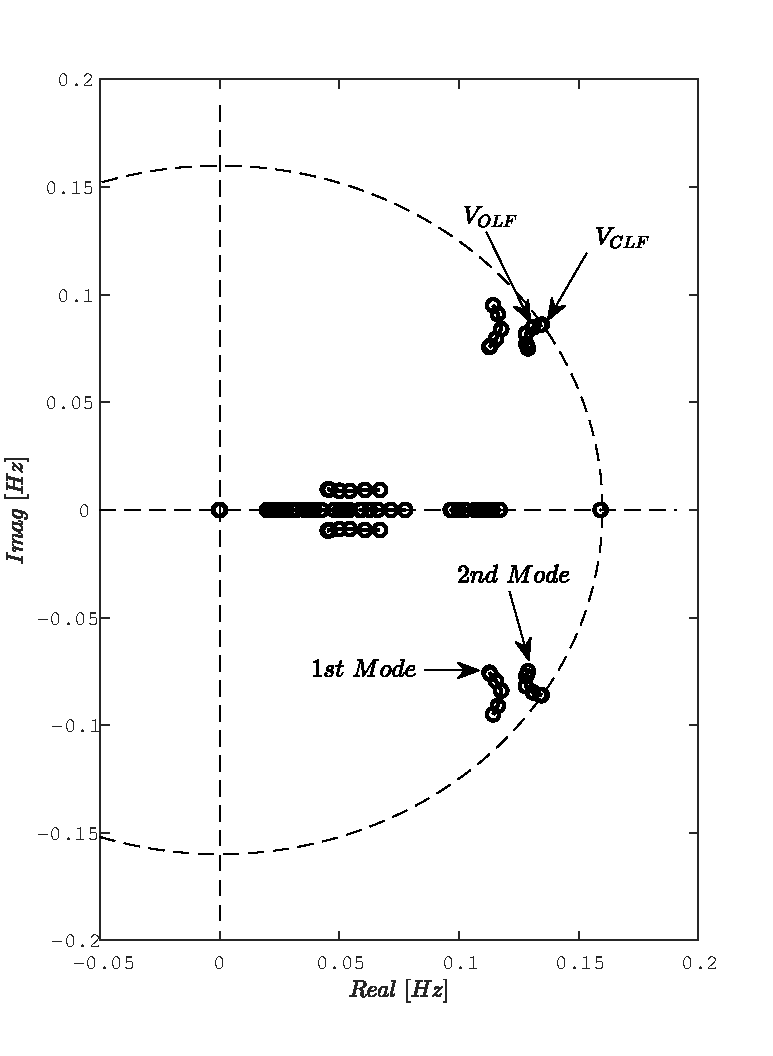
\includegraphics[width=\textwidth]{trabalho-graduacao/capitulos/figures/cap_4/Closed-Loop-Poles/ClosedLoopPoles.pdf}

    \label{fig:ClosedLoop-Poles}
\end{figure}

A avaliação do comportamento dinâmico do sistema em malha fechada também foi realizada a partir de simulações numéricas computacionais. Foram estudadas distintas condições de voo, para velocidades menores, igual e maiores à $V_{OLF}$, todas para condição ISA no nível do mar. As simulações foram realizadas utilizando-se condições iniciais impostas ao primeiro estado, referente ao deslocamento primeiro \gls{GDL}, $h$, emulando uma perturbação em relação à condição de equilíbrio.

\newpage

A Figura \ref{fig:CloseLoopResponse-t0-VOLF} mostra a resposta dinâmica dos \gls{GDL}s do sistema para uma simulação realizada na condição de $V_{OLF}$, para condição inicial $h = 0,127$ m no sistema. Percebe-se que, com a ação do controlador projetado, o sistema é capaz de eliminar a oscilação de \textit{flutter} em malha aberta, cumprindo a regulação do sistema. 

\begin{figure}[ht!]
    \centering
    \caption{Resposta dinâmica em malha fechada, para uma velocidade $V_{\infty} = 29,59$ m/s, com condição inicial não nula no primeiro \gls{GDL} igual à $h=0,127$ m}
    \noindent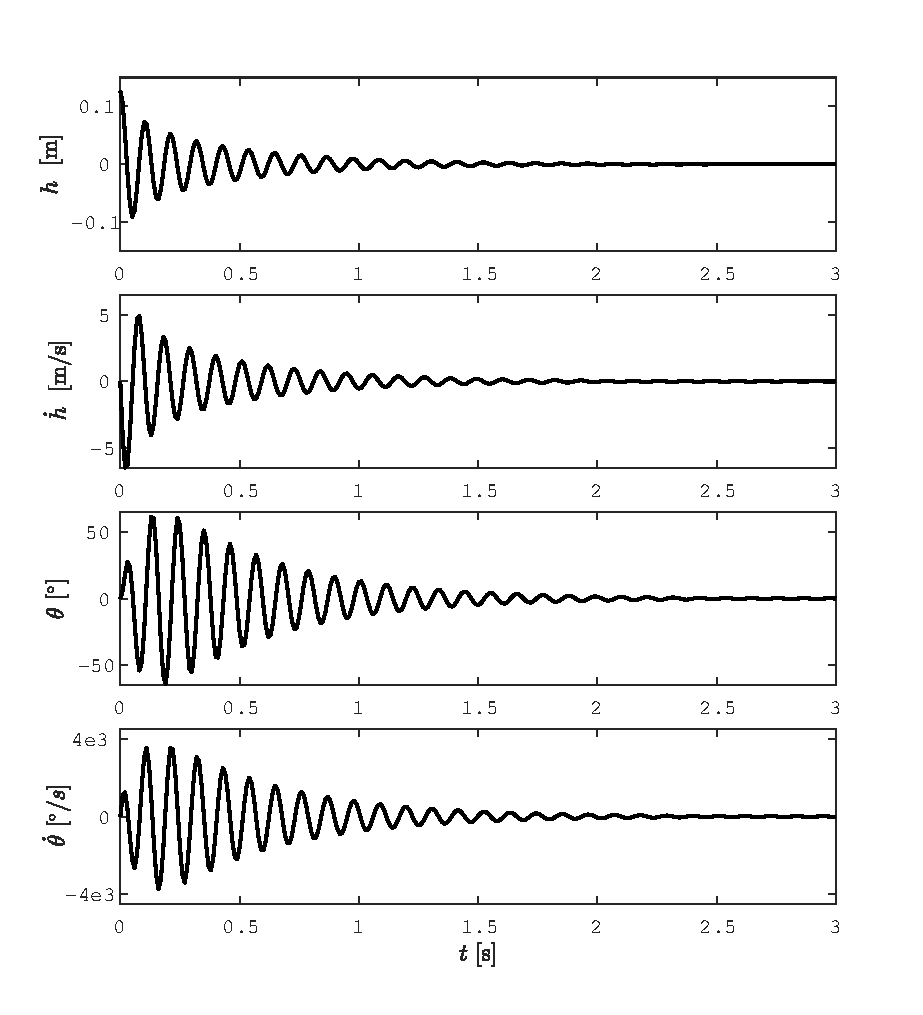
\includegraphics[width=\textwidth]{trabalho-graduacao/capitulos/figures/cap_4/Closed-Loop-Simulation/CLSimulation-VOLF-t0-modes.pdf}
    \label{fig:CloseLoopResponse-t0-VOLF}
\end{figure}


A ação de controle calculada a cada instante de tempo é apresentada na Figura \ref{fig:CloseLoopControl-t0-VOLF}, junto dos estados referentes ao movimento da superfície de controle. Avaliando os resultados, destaca-se o atraso do movimento angular da superfície em relação à entrada calculada pelo controlador, proveniente da dinâmica do atuador. Percebe-se, também, que o sistema apresenta um erro em regime permanente, sendo o a deflexão da superfície de controle não retornando à sua posição inicial, e o sistema assumindo uma nova posição de equilíbrio aeroelástico estático. Como discutido por \textcite{art:Sun-2014}, isso é resultado da não controlabilidade do sistema, conforme apresentado na seção anterior.


\begin{figure}[ht!]
    \centering
    \caption{Ação de controle e estados da superfície de controle, para uma velocidade $V_{\infty} = 29,59$ m/s, com condição inicial não nula no primeiro \gls{GDL} igual à $h=0,127$ m}
    \noindent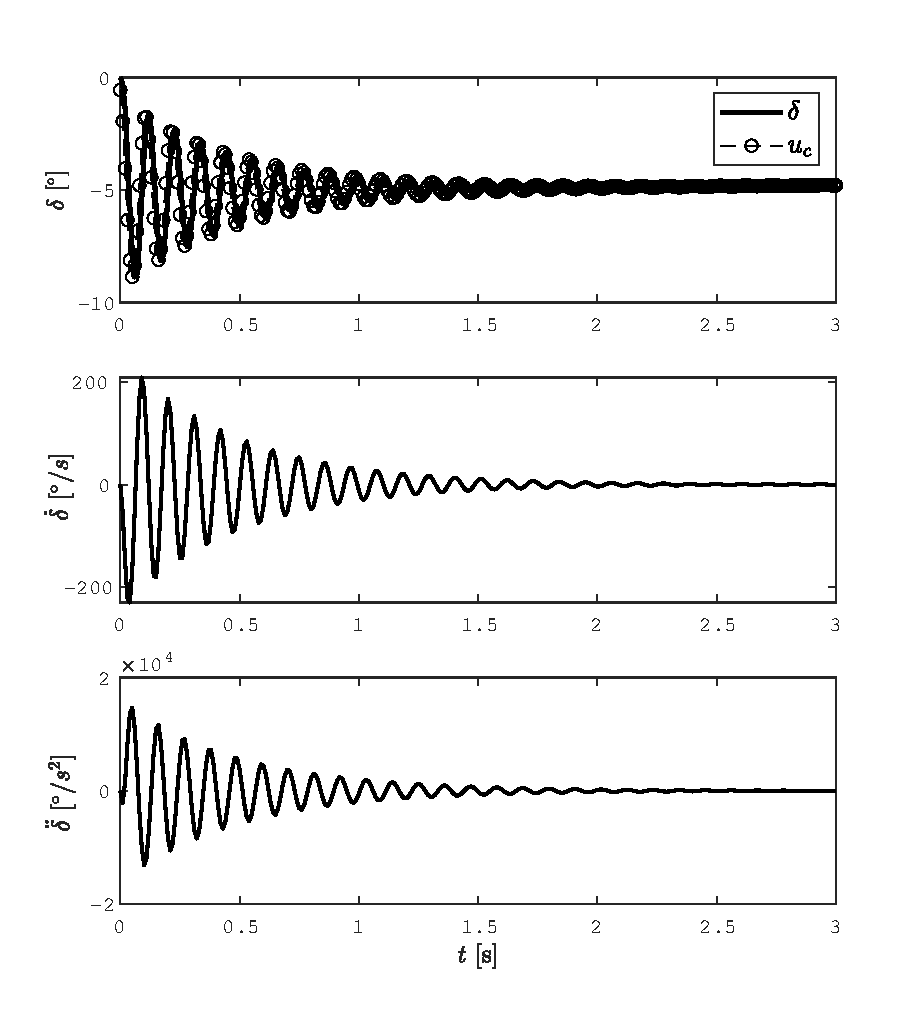
\includegraphics[width=\textwidth]{trabalho-graduacao/capitulos/figures/cap_4/Closed-Loop-Simulation/CLSimulation-VOLF-t0-control.pdf}
    \label{fig:CloseLoopControl-t0-VOLF}
\end{figure}

\newpage
O novo ponto de instabilidade do sistema em malha fechada, $\gls{VCLF}$, também foi avaliado em simulação com uma perturbação no estado inicial. Os resultados são mostrados nas Figuras \ref{fig:CloseLoopResponse-t0-VCLF} e \ref{fig:CloseLoopControl-t0-VCLF}. Apesar da ação do controlador sobre o sistema evitar que a resposta dinâmica divirja, para essa velocidade do escoamento, a estrutura de controle também não é capaz de estabilizar o movimento.

\begin{figure}[ht!]
    \centering
    \caption{Resposta dinâmica em malha fechada, para uma velocidade $V_{\infty} = 31,37$ m/s, com condição inicial não nula no primeiro \gls{GDL} igual à $h=0,127$ m}
    \noindent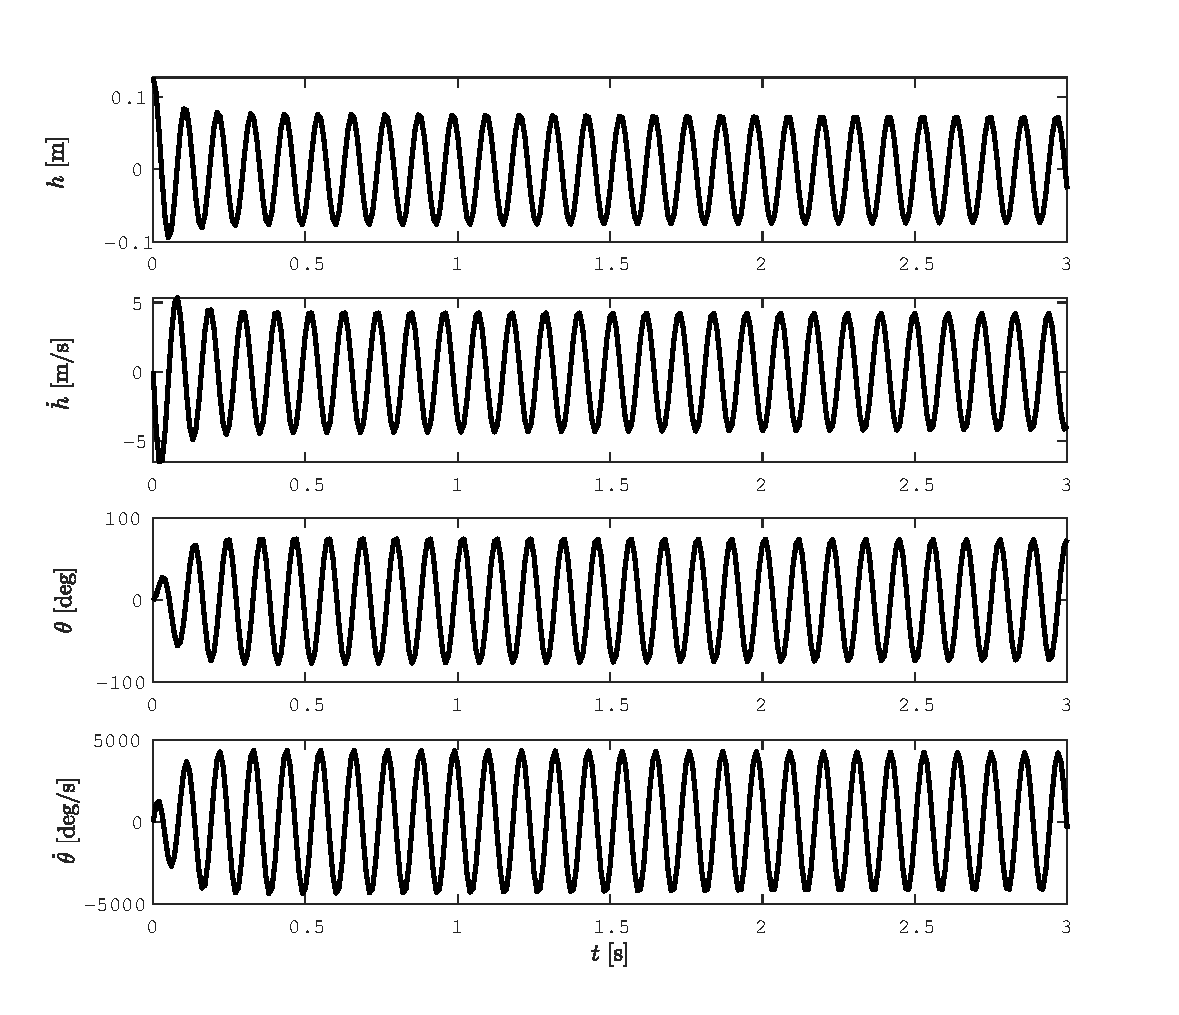
\includegraphics[width=\textwidth]{trabalho-graduacao/capitulos/figures/cap_4/Closed-Loop-Simulation/CLSimulation-VCLF-t0-modes.pdf}

    \label{fig:CloseLoopResponse-t0-VCLF}
\end{figure}

\begin{figure}[ht!]
    \centering
    \caption{Ação de controle e estados da superfície de controle, para uma velocidade $V_{\infty} = 31,37$ m/s, com condição inicial não nula no primeiro \gls{GDL} igual à $h=0,127$ m}
    \noindent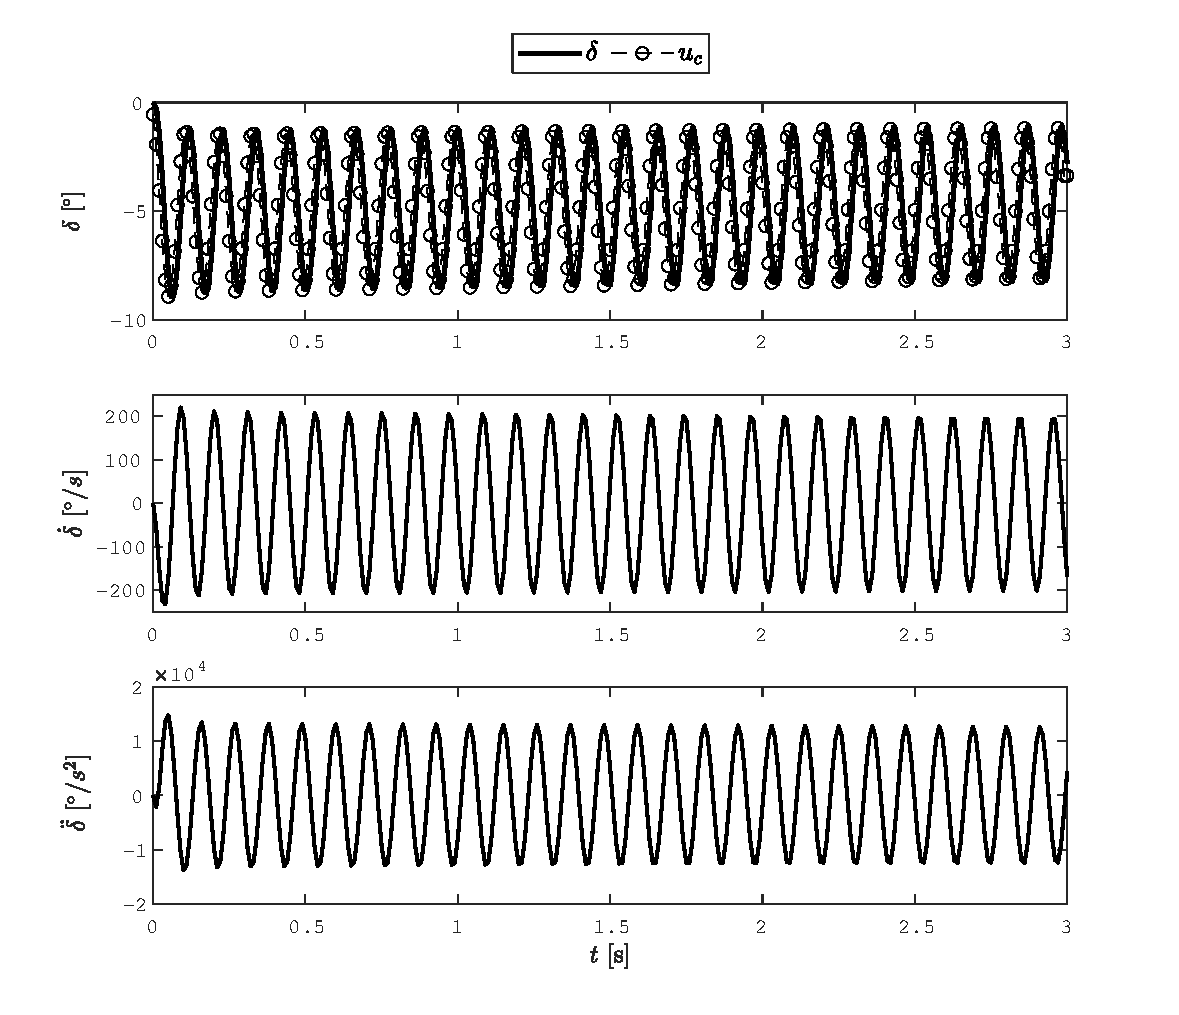
\includegraphics[width=\textwidth]{trabalho-graduacao/capitulos/figures/cap_4/Closed-Loop-Simulation/CLSimulation-VCLF-t0-control.pdf}
    \label{fig:CloseLoopControl-t0-VCLF}
\end{figure}

Avaliou-se também, o efeito da lei de controle implementada em velocidades inferiores à de instabilidade em malha aberta, $V_{OLF}$. Conforme apresentado na Figura \ref{fig:CloseLoopResponse-t0-1000}, a estrutura em malha fechada para o sistema é capaz de reduzir o tempo necessário para os \gls{GDL}s retornarem à posição de equilíbrio. Entretanto, identificou-se que, para velocidades inferiores à $2,50$ m/s, a presença do controlador projetado para a condição de $V_{OLF}$ desestabilizou o sistema, como mostrado pelos resultados de simulação das Figuras \ref{fig:CloseLoopResponse-t0-VLVF} e \ref{fig:CloseLoopControl-t0-VLVF}. Essa característica é explicada pela operação muito longe da condição de projeto do controlador, alinhada ao sistema ser não controlável, resultando na não garantia da robustez da resposta em malha fechada para condições fora da região de projeto. Para referência, são apresentados na Figura \ref{fig:CloseLoopPoles} os polos do sistema em malha fechada para essa condição de instabilidade em velocidades baixas em malha fechada, denominada $\gls{VLVI}$. Percebe-se que os polos referentes aos primeiros modos do sistema, associados aos graus de liberdade da seção típica, estão contidos no círculo unitário, portanto são estáveis para essa condição. O polo instável é dado para frequência nula, e analisando esse dado junto do resultado de simulação podemos concluir que está associado ao movimento da superfície de controle.

\begin{figure}[ht]
    \centering
    \caption{Resposta dinâmica em malha fechada, para uma velocidade $V_{\infty} = 25,0$ m/s, com condição inicial não nula no primeiro \gls{GDL} igual à $h=0,127$ m}
    \noindent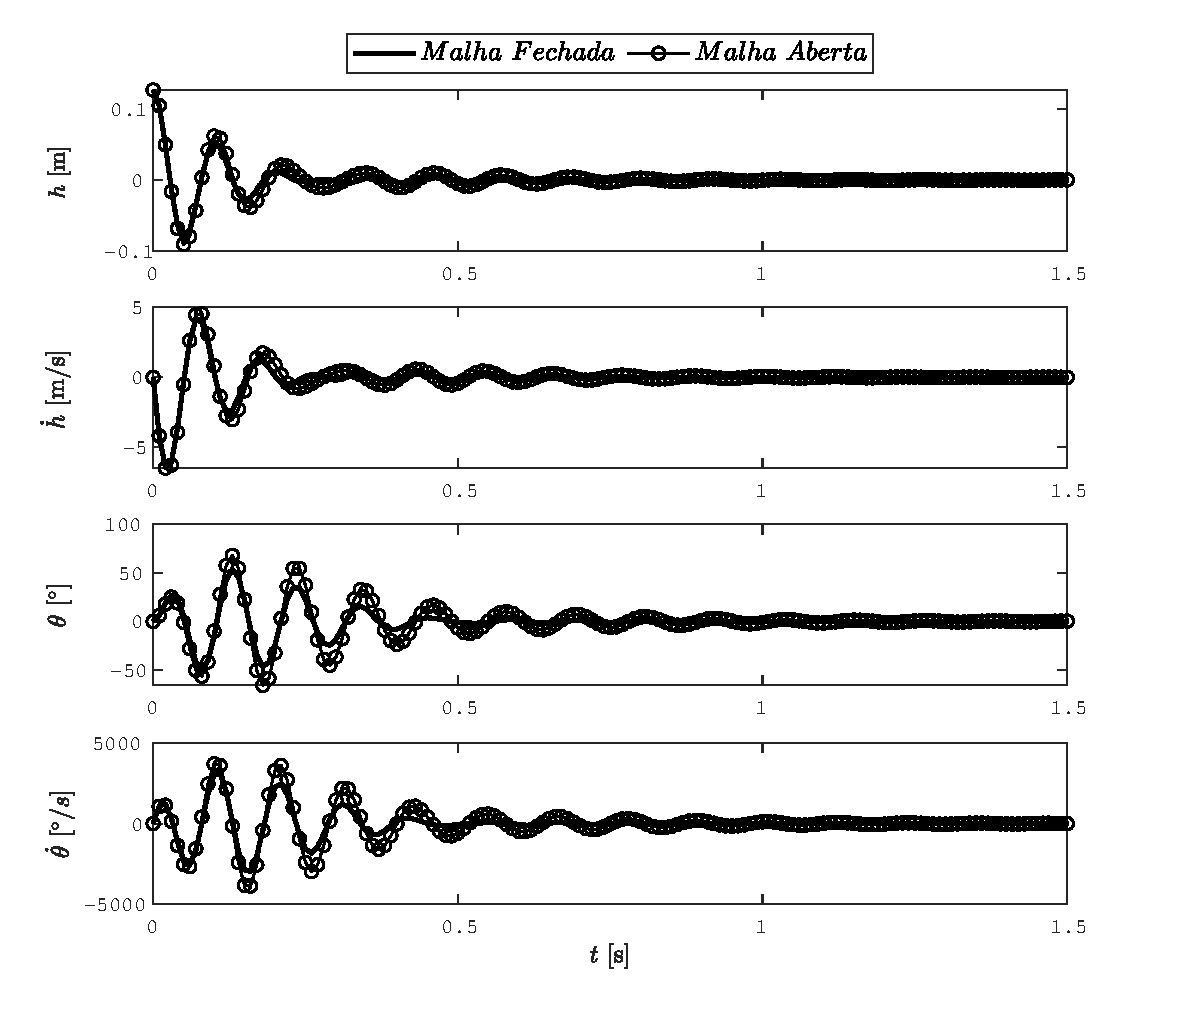
\includegraphics[width=\textwidth]{trabalho-graduacao/capitulos/figures/cap_4/Closed-Loop-Simulation/CLSimulation-1000-t0-modes.pdf}
    \label{fig:CloseLoopResponse-t0-1000}
\end{figure}

Por essa instabilidade estar associada à uma frequência nula, ela é definida como do tipo divergência dinâmica e não \textit{flutter}, como definido por \textcite{book:Wright-Cooper}.

\begin{figure}[ht]
    \centering
    \caption{Resposta dinâmica em malha fechada, para uma velocidade $V_{\infty} = 2,50$ m/s $(\gls{VLVI})$, com condição inicial não nula no primeiro \gls{GDL} igual à $h=0,127$ m}
    \noindent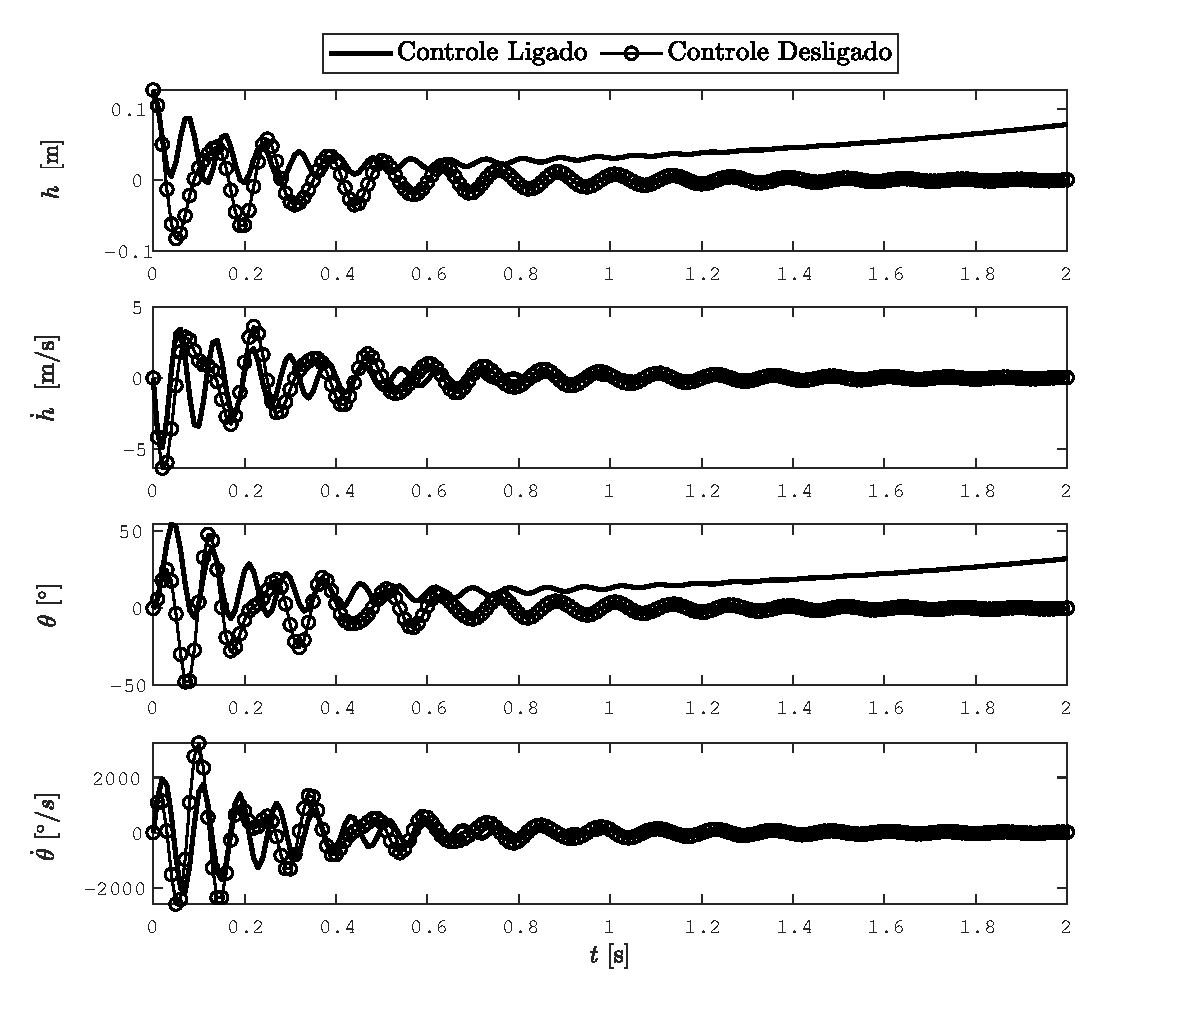
\includegraphics[width=\textwidth]{trabalho-graduacao/capitulos/figures/cap_4/Closed-Loop-Simulation/CLSimulation-VLVF-t0-modes.pdf}
    \label{fig:CloseLoopResponse-t0-VLVF}
\end{figure}

\begin{figure}[ht]
    \centering
    \caption{Ação de controle e estados da superfície de controle, para uma velocidade $V_{\infty} = 2,50$ m/s $(\gls{VLVI})$, com condição inicial não nula no primeiro \gls{GDL} igual à $h=0,127$ m}
    \noindent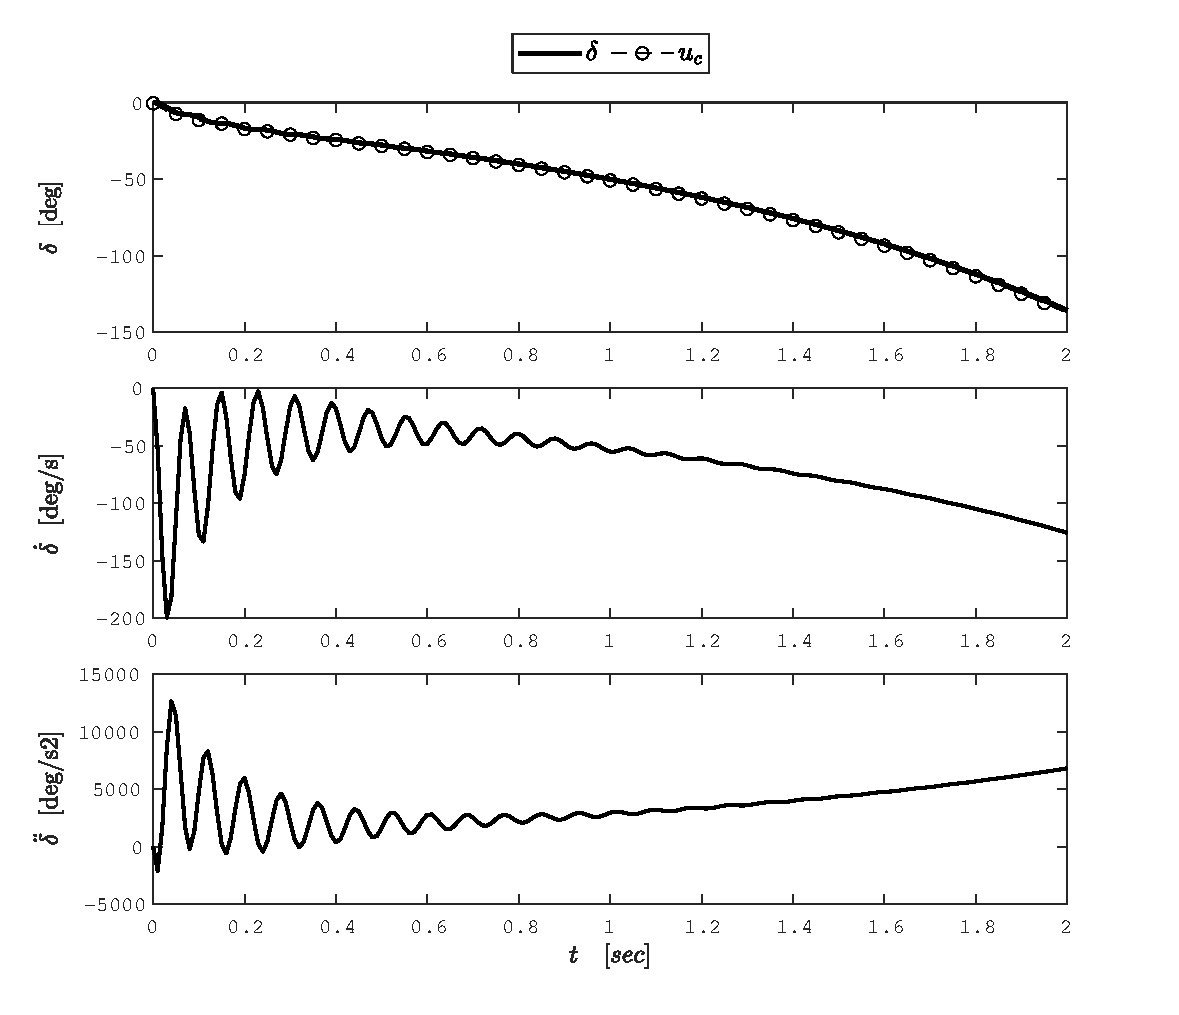
\includegraphics[width=\textwidth]{trabalho-graduacao/capitulos/figures/cap_4/Closed-Loop-Simulation/CLSimulation-VLVF-t0-control.pdf}
    \label{fig:CloseLoopControl-t0-VLVF}
\end{figure}

\begin{figure}[ht]
    \centering
    \caption{Polos em malha fechada para condição $\gls{VLVI}$}
    \noindent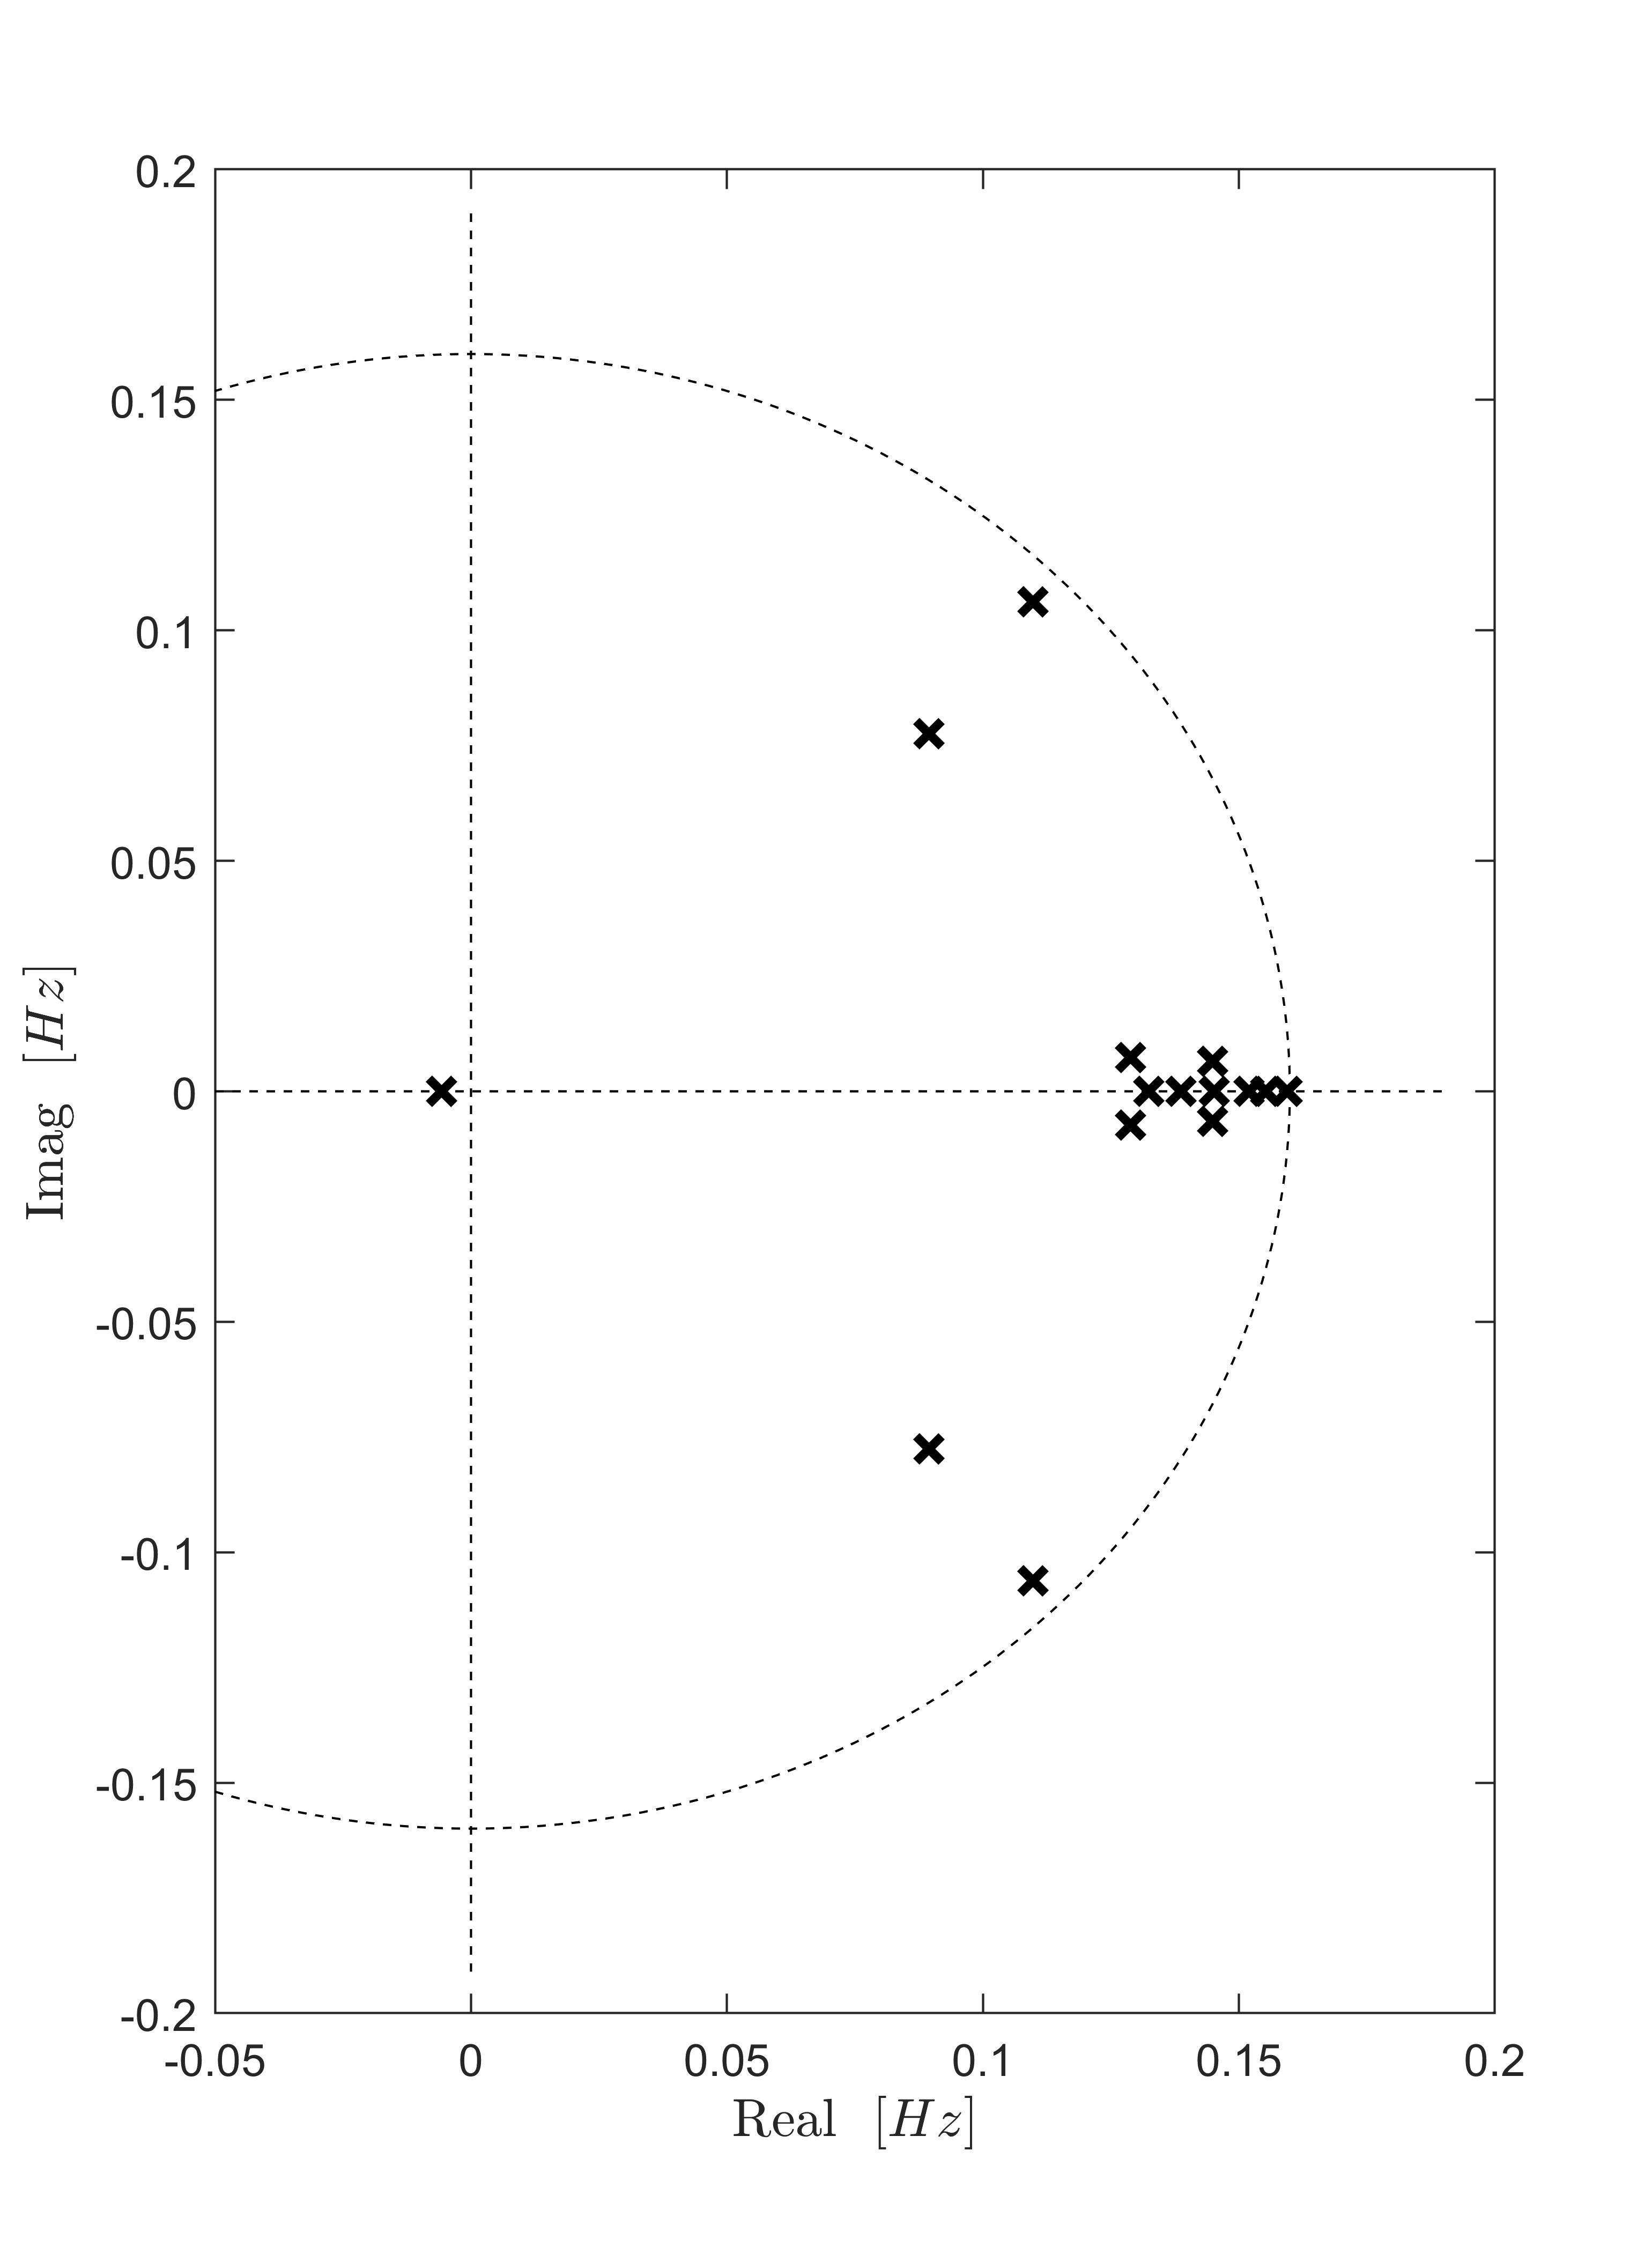
\includegraphics[width=\textwidth]{trabalho-graduacao/capitulos/figures/cap_4/Closed-Loop-Poles/ClosedLoopPoles-VLVF.png}
    \label{fig:CloseLoopPoles}
\end{figure}
